\documentclass[a4paper]{article}

\usepackage[utf8]{inputenc}
\usepackage[T1]{fontenc}
\usepackage[francais]{babel}
\usepackage[a4paper]{geometry}
\usepackage{amsmath}
\usepackage{amssymb}
\usepackage{pdfpages}
\usepackage{float}
\usepackage{wrapfig}
\usepackage{subcaption}
	
\geometry{left=2.75cm, right=2cm, bottom=2cm, top=2cm}

\title{TR Théorie du contrôle - Sujet 2 : Schumacher}
\author{Paul Fraenkel}
\date{}

\sloppy

\begin{document}
	
	\maketitle
	
	\begin{abstract}
		This article presents several modelisations of a minimal time optimal control problem in a constrained environment. Collisions constraints are easily described by non-smooth functions, however, the use of such constraints often leads numerical solver to fail or require a big number of iterations. This work combines different methods for collision constraints [...] to allow a wheeled robot to navigate in an industrial environment without colliding. Different models of the robot are proposed, ranging from a cinematic model, to a dynamic model with centrifugal force limitation. Additionnaly, a model including friction modelisation has been implemented.
	\end{abstract}
	
	\tableofcontents
	
	\part{Introduction}
	Collision detection is a fundamental aspect of autonomous robotics and path planning. In industrial environments such as automated storage facilities, robots are evolving in a challenging environment with many obstacles, and poorly calculated trajectory can lead to serious damage, both for the robot and the environment around it. The company Fives Xcella [...] intends to develop such an automatic storage facility [...]. The solution they came up with uses automatic robots that navigate from storage space to storage space while carrying payloads. One of the limitations of this kinf of system is the fluidity of the robots travel [...]. The rate of the system is limited by robots that need to leave a main lane into a perpendicular sub lane, and slowing down while doing so, thus creating a potential jam. This turn problem constitutes an optimal control problem subect to collisions constraints with the borders of the lanes. This article tackles the broader problem of optimal control of a robot with collision state constraints, using a discretize then optimize approach [...]. The efficiency of three different collisions modelisation between convex polyhedras has been tested with different physice models and four different types of obstacles.
	
	?? Est-ce que je peux prendre les références trouvées dans d'autres articles pour mon article, est-ce que c'est honnête intellectuellement, est-ce du plagiat ?? 
	
	
	
	
	\part{Modelisation of the problem}
	\section{General problem}
	The motivation behind this work is to minimize the "dispearance time" of a robot from a main lane into a perpendicular secondary lane. However, the problem tackled in the following pages is a modified version of the original one. The optimization target is the travel time bewteen a start position and speed and an end position and speed. Because of the small difference between the width of the robot and the width of the secondary lane, the robot must engage itself almost perfectly aligned with the direction lane. Therefore, its position when disapearing is roughly known, and can be defined as the end position of our problem. [figures]
	
	\section{Discretize-then-optimize}
	The problem requires continuous collision checking along a planned trajectory between the robot’s geometric model and the surrounding environment. A substantial body of prior work has introduced differentiable collision constraints for interactions between convex polygons. Such formulations are particularly well suited for evaluating collision avoidance at discrete time instances and can therefore easily be embeded within a discretize-then-optimize approach. Thus, collision-free motion is certified by imposing state constraints at each discretized point along the trajectory.
	
	Nevertheless, in certain configurations, the finite temporal discretization may lead to infeasible or suboptimal solutions, as collisions occurring between discretization nodes are not explicitly captured. These artifacts can affect the convergence of the solver or lead to trajectories that are numericaly feasible but physically invalid. To limit these issues, additional solver tuning or the introduction of additional constraints is often required in order to guide the solver toward a good solution.
	
	
	\paragraph{"Tunneling"}
	This issue is well known in physics simulations that involve fast moving objects, that are simulated at a limited samplerate. Although it is possible, yet complicated, to approximate the volume swept by the object, a much simpler tradeof is to add more points in the simulation. The problem proposed here does not require to be solved in real time, and one can afford to increase the number of discretization points.
	
	\begin{figure}[H]
		\centering
		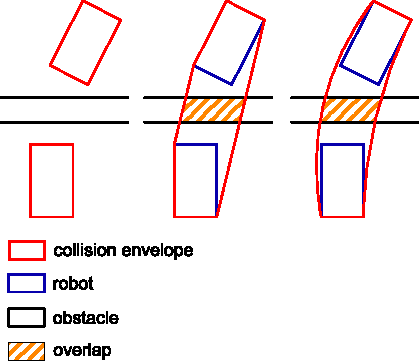
\includegraphics{illustrations/bullet_collision.pdf}
		\caption{Examples of collision envelopes}
		\label{fig:col_env}
	\end{figure}
	
	The general idea of this fix is to reduce the time step between two points. This can be achieved in two ways : firstly by increasing the number of points, or by limiting the maximum time. Trajectories found by the solver that display this kind of issue often go far away from the obstacles to gather speed, which takes a lot of travel time. Solvers find local minima that do not please us. Adding an upper bound to the time obtained by the solver prevents the robot from venturing too far and jumping long distances between two timesteps.
	
	
	\begin{figure}[!h]
		\centering
		\begin{subfigure}{0.45\textwidth}
			\centering
			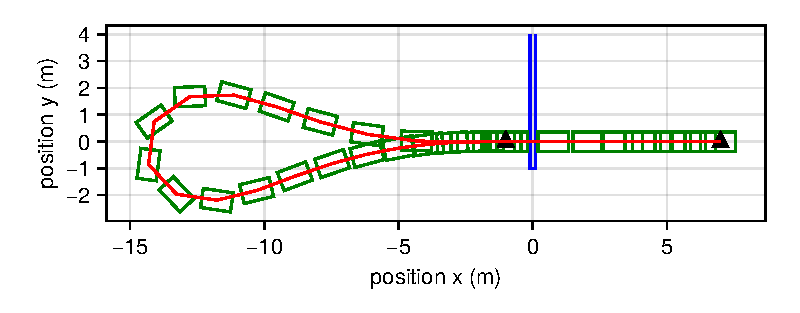
\includegraphics[width=\linewidth]{illustrations/tunneling.pdf}
			\caption{No time limitation}
			\label{fig:tunneling}
		\end{subfigure}
		\begin{subfigure}{0.45\textwidth}
			\centering
			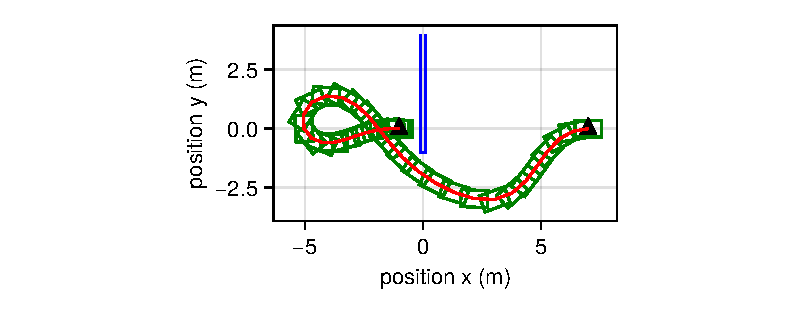
\includegraphics[width=\linewidth]{illustrations/notunneling.pdf}
			\caption{Time limitation}
			\label{fig:notunneling}
		\end{subfigure}
		\caption{Improved solution with time limitation}
	\end{figure}
	
	
	\paragraph{"Corner cliping"}
	This issue arises when the robot makes a turn where one of its front corner might come into contact with another sharp feature of the terrain like a corner. There are two consequencies to this case. First, the trajectory is impossible in reality. During the turn, the robot corner will collide with the terrain corner.. Second, solvers tend to get stuck in local minima and propose solutions that are sub-optimal. For instance, if at some point in the optimization, the trajectory places the corner of the robot at a point on one side, and at the next point on the other side, it is probable that the solver will never exit that state. Thus, the robot might be forced to slow down during the first half before it can accelerate to reach its final destination after the sharp feature.
	
	\begin{figure}[H]
		\centering
		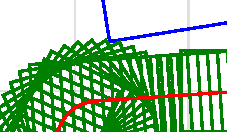
\includegraphics[width=0.5\linewidth]{illustrations/clipping_zoom.pdf}
		\caption{Zoom on corner clipping issue}
		\label{fig:clipping_zoom}
	\end{figure}
	
	\begin{figure}[H]
		\centering
		\begin{subfigure}{0.45\textwidth}
			\centering
			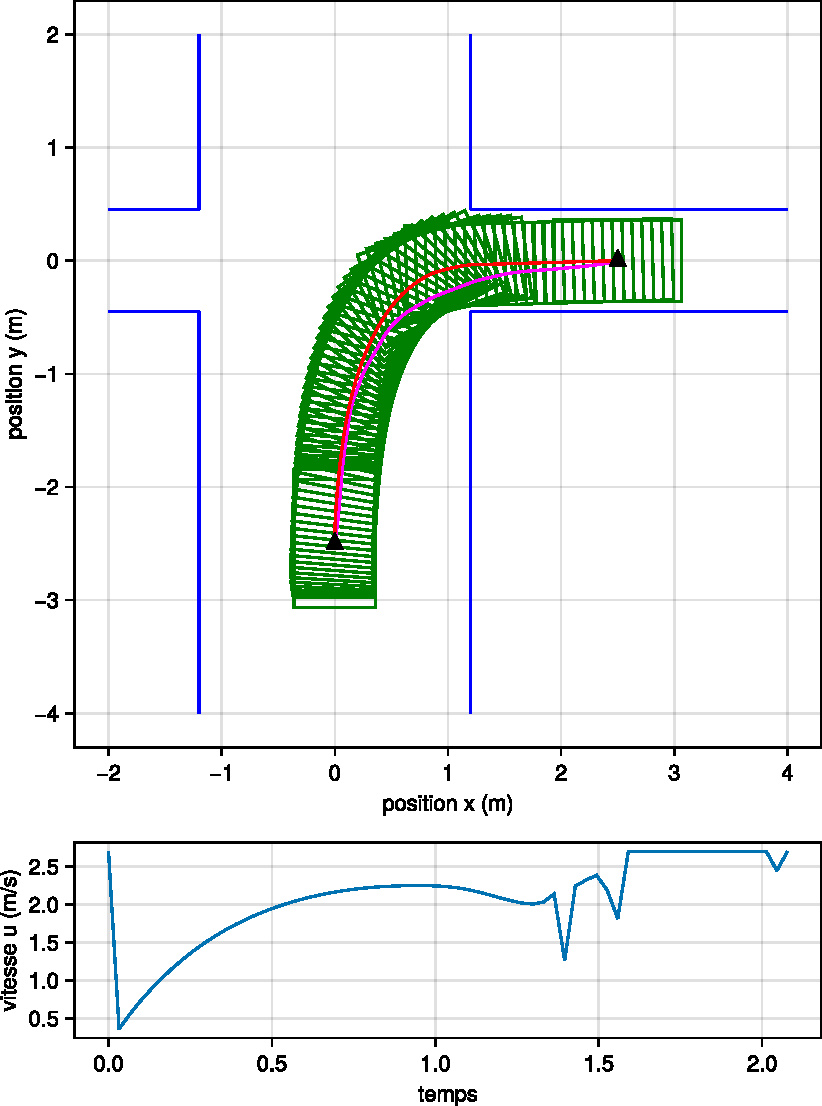
\includegraphics[width=\linewidth]{illustrations/clipping.pdf}
			\caption{Corner clipping}
		\end{subfigure}
		\hspace{1cm}
		\begin{subfigure}{0.45\textwidth}
			\centering
			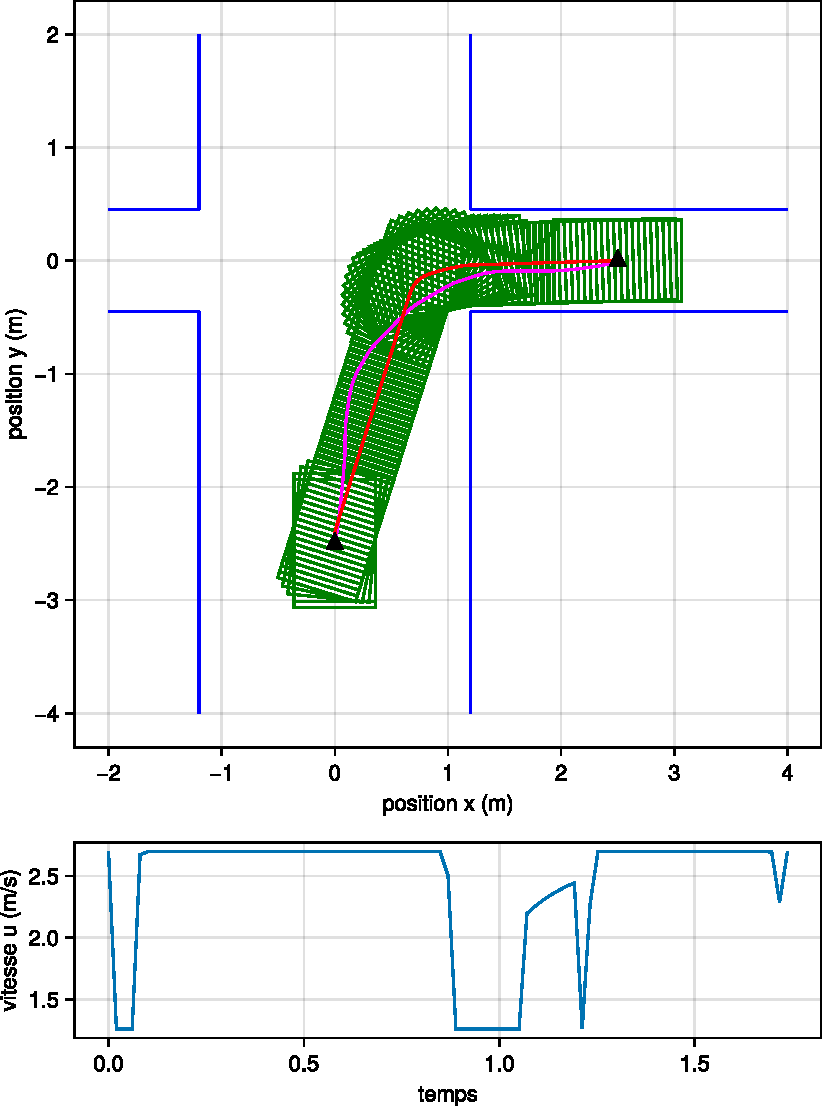
\includegraphics[width=\linewidth]{illustrations/noclipping.pdf}
			\caption{No corner clipping, optimal solution}
		\end{subfigure}
		\caption{Effect of corner clipping on the trajectory}
		\label{fig:clipping}
	\end{figure}
	
	In the above example (fig: \ref{fig:clipping}), the issue was solved by increasing the number of points in the discretization. 
	
	
	\section{Cinematic model}
	
	\section{Brief description of an optimize then discretize method}
	
	\section{Dynamic model}
	
	
	
	
	\part{Constraints on the state}
	Issue with collision detection (usually not differentiable)
	
	\section{Polyhedra representation}
	
	\subsection{Faces}
	\subsection{Vertices}
	
	\section{Methods for collision detection}
	\subsection{2012}
	\subsection{2017}
	\subsection{2023}
	
	
	
	
	\part{Friction modelisation}
	
	\section{Physical model}
	
	\section{Complementarity constraints}
	
	
	
	
	\part{Implementation}
	
	\section{Solver used}
	
	\section{Study cases}
	results ?
	
\end{document}

